\section{最优解的判别}
\label{sec:func-optimality}

有了微分，就可以判别候选。泛函优化的最优解满足什么条件，什么条件又足以断定最优？一阶条件、凸性下的充分性与有限维完全平行；二阶充分性和约束乘子则要额外的前提。

\paragraph{局部极小依赖范数}
在讲条件之前要先说清“局部”。设$J$定义在$\bm{C}$上，若存在$r>0$，使$\lVert u-u^\star\rVert<r$的可行$u$都满足$J(u)\geq J(u^\star)$，称$u^\star$是范数$\lVert\cdot\rVert$下的\term{局部极小点}（local minimizer）。有限维中范数等价，不用说明是哪一个；函数空间中必须说明。

看下面的例子。在$[0,1]$上的Lipschitz函数中，取$u(0)=u(1)=0$，目标
\begin{equation}
 J(u)=\int_0^1\bigl(u'(x)^2-u'(x)^4\bigr)\,\mathrm{d}x.
 \label{eq:func-local-example}
\end{equation}
若用范数$\lVert u\rVert_\infty+\lVert u'\rVert_\infty$，当它小于$1$时$\lvert u'\rvert<1$，被积函数非负，$J\geq0=J(0)$，所以$u=0$是局部极小点。

若只用上确界范数$\lVert u\rVert_\infty$，取图~\ref{fig:func-zigzag-local}(a)的锯齿：$k$个相同的齿，斜率$\pm2$。它的高度是$1/k$，$k$越大越贴近零函数；而被积函数处处等于$4-16=-12$，
\[
 \lVert u\rVert_\infty=\frac1k,\qquad J(u)=-12.
\]
所以$u=0$在上确界范数下不是局部极小点。前一种范数把导数也算进“接近”，这样的扰动被排除了。

\begin{BookInlineFigure}
  \centering
  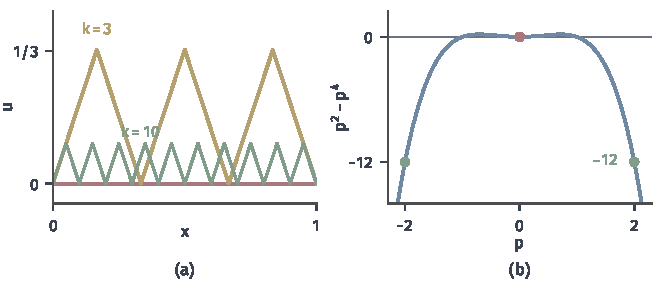
\includegraphics[width=112mm]{figures/05-optimization/08-functional-optimization/matplotlib/func-zigzag-local/figure.pdf}
  \caption{局部极小依赖范数。(a)红线$u=0$附近的锯齿，斜率$\pm2$，黄色$k=3$，绿色$k=10$；上确界距离$1/k$趋于零，而导数始终等于$\pm2$。(b)被积函数$p^2-p^4$：$p=0$是局部极小（红点），大斜率处（绿点）取值$-12$。}
  \label{fig:func-zigzag-local}
\end{BookInlineFigure}

\paragraph{一阶必要条件}
第~\ref{chap:constrained-optimality}章用可行方向得到一阶条件，这里的推理逐字相同，因为它只看一条线段。称$\eta$是$\bm{C}$在$u$处的\term{可行方向}（feasible direction），若$t>0$充分小时$u+t\eta\in\bm{C}$。

\begin{theorem}[一阶必要条件]
\label{thm:func-first-order}
设$u^\star$是$J$在$\bm{C}$上某范数下的局部极小点，$\eta$是$u^\star$处的可行方向，方向导数存在。则
\begin{equation}
 J'(u^\star;\eta)\geq0.
 \label{eq:func-first-order}
\end{equation}
进一步，设$J$在$u^\star$处沿所需方向Gâteaux可微。若$\bm{C}=u_0+\bm{V}$，$\bm{V}$是子空间，则
\begin{equation}
 DJ(u^\star)[\eta]=0\qquad(\eta\in\bm{V}).
 \label{eq:func-stationary}
\end{equation}
若$\bm{C}$是凸集，则
\begin{equation}
 DJ(u^\star)[v-u^\star]\geq0\qquad(v\in\bm{C}).
 \label{eq:func-variational-inequality}
\end{equation}
\end{theorem}

\begin{proof}
$t>0$充分小时，$u^\star+t\eta$可行，且与$u^\star$的距离$t\lVert\eta\rVert$小于$r$，所以
\[
 \frac{J(u^\star+t\eta)-J(u^\star)}{t}\geq0.
\]
令$t\downarrow0$得到式~\eqref{eq:func-first-order}。子空间情形中$\eta$和$-\eta$都是可行方向，由线性得到两个相反的不等式，于是式~\eqref{eq:func-stationary}成立。凸集情形中$v-u^\star$是可行方向，代入式~\eqref{eq:func-first-order}。
\end{proof}

式~\eqref{eq:func-stationary}称为驻定条件，满足它的点称为驻点。若$\bm{V}$上有Hilbert结构，它就是$\nabla_{\bm{V}}J(u^\star)=0$。注意这里的梯度是$\bm{V}$内的，$X$内的梯度只需与$\bm{V}$正交，这和等式约束问题中梯度落在约束法方向上相同。式~\eqref{eq:func-variational-inequality}是第~\ref{chap:constrained-optimality}章的变分不等式。

\paragraph{凸性下的充分性}
凸性让局部信息变成全局结论。若$J$是凸泛函，沿线段的一元函数$\phi$是凸的，切线在下方，由此得到下面的结论。

\begin{theorem}[凸问题的充分条件]
\label{thm:func-convex-sufficient}
设$\bm{C}$是凸集，$J$在$\bm{C}$上是凸的，在$u^\star\in\bm{C}$处有$J'(u^\star;v-u^\star)\geq0$，对每个$v\in\bm{C}$成立。则$u^\star$是全局最优解。若$J$严格凸，它是唯一的最优解。
\end{theorem}

\begin{proof}
任取$v\in\bm{C}$，令$\phi(t)=J(u^\star+t(v-u^\star))$，$t\in[0,1]$。由凸性，$t\in(0,1]$时
\[
 \frac{\phi(t)-\phi(0)}{t}\leq\phi(1)-\phi(0).
\]
令$t\downarrow0$，左端趋于$J'(u^\star;v-u^\star)\geq0$，所以$J(v)\geq J(u^\star)$。

若$J$严格凸，并有另一最优解$v\neq u^\star$，则中点的目标值严格小于$J^\star$，矛盾。
\end{proof}

对$E$，式~\eqref{eq:func-energy-expansion}中的余项$\frac12\lVert\eta\rVert_{H^1}^2$在$\eta\neq0$时严格为正。所以$E$严格凸，驻点若存在，就是唯一的全局最优解。第~\ref{sec:func-existence}节证明了存在性，这里证明了驻点即最优，两者合起来，驻定方程的解就是答案。

\paragraph{二阶变化}
没有凸性时，要看二阶信息。沿直线，$\phi''(0)$就是二阶变化。

\begin{definition}[二阶变分]
\label{def:func-second-variation}
若$\phi(t)=J(u+t\eta)$在$t=0$的邻域内二阶可导，称
\begin{equation}
 \delta^2J(u;\eta)=\phi''(0)
 \label{eq:func-second-variation}
\end{equation}
为$J$在$u$处沿$\eta$的\term{二阶变分}（second variation）。
\end{definition}

若$u^\star$是子空间方向上的局部极小点，则$\phi$在$t=0$处局部极小，所以$\phi'(0)=0$，并有$\phi''(0)\geq0$。这是二阶必要条件：$\delta^2J(u^\star;\eta)\geq0$，对每个$\eta\in\bm{V}$成立。

\paragraph{用坐标看二阶变分}
目标~\eqref{eq:func-rho}是二次的，$\phi(t)=t^2J_\rho(\eta)$，所以
\[
 \delta^2J_\rho(0;\eta)=\int_0^1\bigl(\eta'^2-\rho\eta^2\bigr)\,\mathrm{d}x.
\]
把$\eta\in H^1_0(0,1)$按标准正交基$\sqrt2\sin(k\pi x)$展开，系数为$a_k$。由Parseval等式，$\lVert\eta\rVert_2^2=\sum_ka_k^2$。

对$\eta'$，它按$\sqrt2\cos(k\pi x)$展开的系数，由分部积分（边界项因$\eta$在端点为零而消失）等于$k\pi a_k$；它与常数函数的内积是$\eta(1)-\eta(0)=0$。所以$\lVert\eta'\rVert_2^2=\sum_k(k\pi)^2a_k^2$。三角函数系的完备性可参考\BookChapterRef{chap:fourier-transform}{卷四第14章“Fourier变换”}。代入得到
\begin{equation}
 \delta^2J_\rho(0;\eta)=\sum_{k=1}^\infty\bigl((k\pi)^2-\rho\bigr)a_k^2.
 \label{eq:func-spectrum}
\end{equation}

这是无限维中的对角二次型，图~\ref{fig:func-spectrum}(a)是$\rho=15$时的对角元。只有$k=1$为负，所以$u=0$是鞍点。对角元有下界但无上界，这是有限维Hessian没有的现象：图~\ref{fig:func-spectrum}(b)中，把问题离散后，最大特征值约为$4n^2$，随网格加密趋于无穷，最小特征值停在$\pi^2$附近。

\begin{BookInlineFigure}
  \centering
  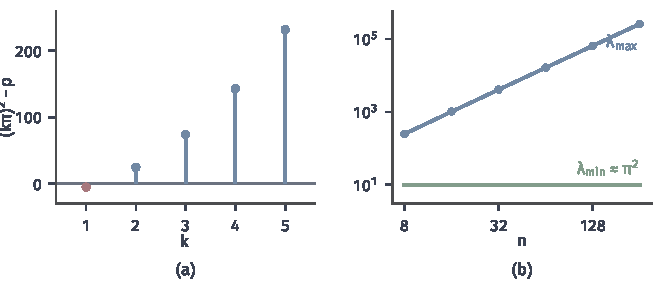
\includegraphics[width=112mm]{figures/05-optimization/08-functional-optimization/matplotlib/func-spectrum/figure.pdf}
  \caption{目标~\eqref{eq:func-rho}的二阶信息。(a)$\rho=15$时式~\eqref{eq:func-spectrum}的对角元，红色为负曲率方向$k=1$。(b)二阶差分矩阵的最大特征值（蓝）随段数$n$按$4n^2$增长，最小特征值（绿）停在$\pi^2$附近，所以$L^2$意义下没有有限的光滑常数$L$。}
  \label{fig:func-spectrum}
\end{BookInlineFigure}

由式~\eqref{eq:func-spectrum}可以读出全部结论。$\rho<\pi^2$时每个对角元为正，$J_\rho$严格凸，$u=0$是唯一的最优解。$\rho=\pi^2$时$t\sin\pi x$全是最优解，解不唯一。$\rho>\pi^2$时目标无下界。这也给出了精确的Poincaré不等式：
\[
 \lVert\eta'\rVert_2^2\geq\pi^2\lVert\eta\rVert_2^2.
\]

\paragraph{处处为正不够}
有限维中，Hessian正定就足以保证严格局部极小，因为单位球面紧，正定函数在其上有正的最小值$\mu$。无限维中球面不紧，这个最小值可以是$0$。

在$\ell^2$上，也就是把函数看成坐标序列，令
\[
 J(\bm{a})=\sum_{k=1}^\infty\Bigl(\frac{a_k^2}{k^2}-a_k^4\Bigr).
\]
由$\sum_ka_k^4\leq\lVert\bm{a}\rVert_2^4$，$J$处处有限。在原点，$J$的一阶微分为零，二阶变分$\delta^2J(\bm{0};\bm{\eta})=2\sum_k\eta_k^2/k^2$，对每个$\bm{\eta}\neq\bm{0}$都是正的。

但取只有第$k$个坐标非零的点$\bm{a}^{(k)}=\frac2k\bm{e}_k$，有
\[
 \lVert\bm{a}^{(k)}\rVert_2=\frac2k\to0,\qquad J(\bm{a}^{(k)})=\frac{4}{k^4}-\frac{16}{k^4}=-\frac{12}{k^4}<0.
\]
所以原点不是局部极小点。曲率$2/k^2$沿高频坐标趋于零，四次项就占了上风。要恢复有限维的结论，必须要求曲率有统一的正下界。

\begin{theorem}[二阶充分条件]
\label{thm:func-second-sufficient}
设$\bm{C}=u_0+\bm{V}$，$J$在$u^\star\in\bm{C}$的邻域内二阶连续Fréchet可微，$DJ(u^\star)$在$\bm{V}$上为零，且存在$\mu>0$使
\begin{equation}
 D^2J(u^\star)[\eta,\eta]\geq\mu\lVert\eta\rVert^2\qquad(\eta\in\bm{V}).
 \label{eq:func-coercive-second}
\end{equation}
则$u^\star$是所用范数下的严格局部极小点。
\end{theorem}

\begin{proof}
由连续性，取$r>0$，使$\lVert v-u^\star\rVert<r$时$\lVert D^2J(v)-D^2J(u^\star)\rVert\leq\mu/2$。对$\eta\in\bm{V}$，$0<\lVert\eta\rVert<r$，用带积分余项的Taylor公式，一阶项为零，
\[
 J(u^\star+\eta)-J(u^\star)=\int_0^1(1-\tau)D^2J(u^\star+\tau\eta)[\eta,\eta]\,\mathrm{d}\tau.
\]
被积式中的二阶微分不小于$\mu\lVert\eta\rVert^2-\frac\mu2\lVert\eta\rVert^2$，所以
\[
 J(u^\star+\eta)-J(u^\star)\geq\frac{\mu}{4}\lVert\eta\rVert^2>0.
\]
\end{proof}

上面的$\ell^2$反例不满足式~\eqref{eq:func-coercive-second}。而$J_\rho$在$0\le\rho<\pi^2$时满足它：由式~\eqref{eq:func-spectrum}，在范数$\lVert\eta'\rVert_2$下，$\mu=1-\rho/\pi^2$。条件是否成立同样依赖范数：同一个二阶变分在$H^1$范数下是强制的，在更强的范数下可能不是。

\paragraph{约束乘子}
若约束不是仿射的，第~\ref{chap:constrained-optimality}章的乘子法则还成立吗？有限个约束时答案是肯定的，因为证明可以化归到有限维。

\begin{theorem}[有限个等式约束的乘子法则]
\label{thm:func-multiplier}
设$X$是Banach空间，$u^\star$是$J$在约束$h_j(u)=0$（$j=1,\ldots,p$）下某范数的局部极小点。设$J,h_1,\ldots,h_p$在$u^\star$的邻域内连续Fréchet可微，且$Dh_1(u^\star),\ldots,Dh_p(u^\star)$线性无关。则存在唯一的$\bm{\nu}\in\mathbb{R}^p$，使
\begin{equation}
 DJ(u^\star)+\sum_{j=1}^p\nu_jDh_j(u^\star)=0\quad\text{于}\ X^*.
 \label{eq:func-multiplier}
\end{equation}
\end{theorem}

\begin{proof}
\emph{选取补方向。}由线性无关，存在$e_1,\ldots,e_p\in X$，使$Dh_i(u^\star)[e_j]$当$i=j$时为$1$，否则为$0$。记$\bm{N}$为全部$Dh_j(u^\star)$的公共零空间。

\emph{化到有限维。}固定$\eta\in\bm{N}$，考虑从$\mathbb{R}\times\mathbb{R}^p$到$\mathbb{R}^p$的映射
\[
 \Psi_j(t,\bm{s})=h_j\Bigl(u^\star+t\eta+\sum_{i=1}^ps_ie_i\Bigr).
\]

在原点$\bm{\Psi}$取零，对$\bm{s}$的Jacobi矩阵是单位阵。由隐函数定理，存在$\bm{s}(0)=\bm{0}$的$C^1$函数$\bm{s}(t)$，使约束沿$t$始终成立。

对$t$求导，并用$Dh_j(u^\star)[\eta]=0$，得到
\[
 \bm{s}'(0)=\bm{0}.
\]

\emph{沿可行曲线求导。}令$w(t)=u^\star+t\eta+\sum_is_i(t)e_i$，它可行，$w(0)=u^\star$，$w'(0)=\eta$。一元函数$J(w(t))$在$t=0$处局部极小，所以导数为零，即$DJ(u^\star)[\eta]=0$。

\emph{写出乘子。}令$\nu_j=-DJ(u^\star)[e_j]$。对任意$v\in X$，$v-\sum_jDh_j(u^\star)[v]\,e_j$属于$\bm{N}$，代入上一步得到
\[
 DJ(u^\star)[v]=-\sum_{j=1}^p\nu_jDh_j(u^\star)[v].
\]
这就是式~\eqref{eq:func-multiplier}。唯一性由线性无关得到。
\end{proof}

关键在于约束只有有限个，隐函数定理只用在$\mathbb{R}^p$上。条件中的连续Fréchet可微和线性无关都依赖所选的空间。

\paragraph{一个可以手算的乘子}
一根两端固定的细线绕过中点处高度为$1$的钉子。写成问题，就是
\[
 \min\ \frac12\int_0^1u'(x)^2\,\mathrm{d}x,\qquad u\in H^1_0(0,1),\quad u(\tfrac12)\geq1.
\]
点值读取在$H^1$中连续，由式~\eqref{eq:func-point-bound}，这个约束是良定义的。候选是图~\ref{fig:func-peg}(a)的折线$u^\star=2\min\{x,1-x\}$。

直接计算微分：把积分在$x=\frac12$处分开，
\[
 DJ(u^\star)[\eta]=2\int_0^{1/2}\eta'\,\mathrm{d}x-2\int_{1/2}^1\eta'\,\mathrm{d}x=4\,\eta\bigl(\tfrac12\bigr).
\]
可行集是凸集。对可行的$v$，有$v(\frac12)\geq1=u^\star(\frac12)$，所以
\[
 DJ(u^\star)[v-u^\star]=4\bigl(v(\tfrac12)-1\bigr)\geq0.
\]
由定理~\ref{thm:func-convex-sufficient}，$u^\star$是全局最优解，$J^\star=\frac12\cdot4=2$。

\begin{BookInlineFigure}
  \centering
  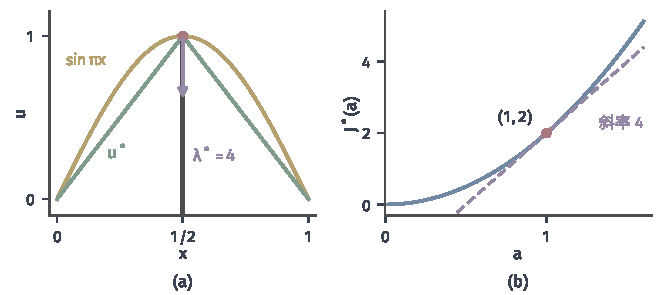
\includegraphics[width=112mm]{figures/05-optimization/08-functional-optimization/matplotlib/func-peg/figure.pdf}
  \caption{钉子问题。(a)深灰竖线是钉子，绿色折线是最优解，黄色$\sin\pi x$是另一个可行候选（能量$\pi^2/4\approx2.47$，大于$2$），紫色箭头表示乘子$\lambda^\star=4$。(b)钉子高度为$a$时的最优值$J^\star(a)=2a^2$，$a=1$处切线（紫色虚线）的斜率等于乘子。}
  \label{fig:func-peg}
\end{BookInlineFigure}

把约束写成$g(u)=1-u(\frac12)\leq0$，于是$Dg[\eta]=-\eta(\frac12)$。平稳条件$DJ(u^\star)+\lambda Dg=0$给出乘子
\[
 \lambda^\star=4\geq0.
\]
乘子仍是影子价格。钉子高度为$a$时，最优解是$2a\min\{x,1-x\}$，最优值是$J^\star(a)=2a^2$，在$a=1$处的导数正是$4$，见图~\ref{fig:func-peg}(b)。把高度抬高一点，能量按每单位高度$4$增加。

这个乘子也可以用梯度来读。在内积$\int v'\eta'$下，读取$\eta\mapsto\eta(\frac12)$的梯度是$w=\frac12\min\{x,1-x\}$，因为$\int_0^1w'\eta'\,\mathrm{d}x=\eta(\frac12)$。而$\nabla J(u^\star)=u^\star=4w$。目标的梯度等于乘子乘以约束的梯度，这与有限维的几何完全相同。

\paragraph{乘子的适用前提}
上面的例子只有一个约束。若要求$u(x)\geq\psi(x)$对每个$x$成立，约束就有无穷多个，定理~\ref{thm:func-multiplier}用不上。乘子要变成对偶空间中的元素，它通常不是函数。把钉子看成这种情形，乘子是中点处的点质量$4\delta_{1/2}$，$u'$在钉子处恰好跳变$-4$。

无穷约束下乘子的存在，需要Slater型条件，也就是可行集在合适拓扑中有内点。这时拓扑的选择又起决定作用：$L^2$中非负函数组成的锥没有内点，因为从任何非负函数减去一个窄而高的尖峰，都可以用任意小的$L^2$范数变成在一小段上为负。而$C[0,1]$中$u\geq\varepsilon>0$的函数是内点。一维时$H^1$的范数控制上确界，内点也存在；高维时这一点不再成立，需要在具体问题中重新论证。

所以，有限维的乘子法则搬到函数空间时要检查三件事：约束是有限个还是无穷个，约束在所选范数下是否可微，约束规范在所选拓扑下是否成立。
